\documentclass{sig-alternate}
\usepackage[english]{babel}
\usepackage{supertabular}
\usepackage[utf8]{inputenc}
\usepackage[T1]{fontenc}
\usepackage{booktabs}
\usepackage{amsfonts}
\setlength{\heavyrulewidth}{1.2pt}
\setlength{\lightrulewidth}{0.7pt}
\DeclareMathOperator*{\argmin}{argmin}

\begin{document}



\title{Deriving Item Features Relevance from Past User Interactions}

\numberofauthors{4}
\author{
\and
\and
\and
\alignauthor
Leonardo Cella\\
       \email{leonardo.cella@mail.polimi.it}\\
       \affaddr{Politecnico di Milano}\\
       \and
       \and
       \and
\alignauthor
Stefano Cereda\\
       \email{stefano1.cereda@mail.polimi.it}\\
       \affaddr{Politecnico di Milano}\\
\and
\and
\and
\and
\alignauthor
Massimo Quadrana\\
       \email{massimo.quadrana@polimi.it}\\
       \affaddr{Politecnico di Milano}\\
       \and
       \and
\alignauthor
Paolo Cremonesi\\
       \email{paolo.cremonesi@polimi.it}\\
       \affaddr{Politecnico di Milano}\\
}
\maketitle

\begin{abstract}
Item-based recommender systems suggest products based on the
similarities between items computed either from past user preferences
(collaborative filtering) or from item content features (contentbased 
filtering). Collaborative filtering has been proven to outperform 
content-based filtering in a variety of scenarios. However, in
item cold-start, collaborative filtering cannot be used directly since
past user interactions are not available for the newly added items.
Hence, content-based filtering is usually the only viable option left.


In this paper we propose a novel feature-based machine learning
model that addresses the item cold-start problem by jointly exploiting
item content features and past user preferences. The model
learns the relevance of each content feature from the collaborative
item similarity, hence allowing to embed collaborative knowledge
into a purely content-based algorithm. In our experiments, the
proposed approach outperforms classical content-based filtering
on an enriched version of the Netflix dataset, showing that collaborative
knowledge can be effectively embedded into content-based
approaches and exploited in item cold-start recommendation.

\end{abstract}

\section{Introduction}

Item-based algorithms are widespread methods for recommending
relevant items to users. Because predictions rely on the
computation of similarities between pairs of items, they have good
runtime performance and their recommendations are easy to explain.
Collaborative Filtering (CF) similarities usually leads to good
predictive accuracy, especially if trained with regard to suitable optimization
objective functions. The downside of CF algorithms
is that similarities are only available for items with a – possibly
large – number of ratings. Thus for entirely new items – i.e., ones
that have no ratings – CF methods are not capable of computing
recommendations. Moreover, CF are biased toward popular Block-
buster items, thus reducing the chances of novel recommendations.
This happens because algorithms are trained (e.g., tuned) to achieve
the best performance in terms of available ratings. This creates the
rich-get-richer effect for popular items, which results in reducing
the coverage of recommendations.


The new-item problem can be solved by using Content-Based
Filtering methods (CBF). CBF requires that items are represented
via a set of features – or attributes – that capture their intrinsic
characteristics. The quality of CBF is severely limited by three
factors \cite{4}:

\begin{itemize}
\item quality is linked to the availability of a number of significant,
well-structured, editorial-generated attributes (such
as genres, actors, directors in the movie domain); however,
many recommender systems base their recommendations
on unstructured, user-generated attri-butes (i.e., tags, reviews)
most of which are noisy or scarcely relevant;
\end{itemize}

\begin{itemize}
\item recommendations to each user do not use the ratings of
other users, therefore ignoring potentially useful collaborative
information;
\end{itemize}

\begin{itemize}
\item recommended items are similar to previously rated 
it-ems,
thus reducing diversity of recommendations.
\end{itemize}


Because of these limitations, a significant challenge to address
with CBF is feature weighting, i.e., how to identify how much a
feature is important in defining the perceived similarity between
items.

Feature weighting can be viewed as an extension of the feature
selection problem, where the goal is to provide an evaluation measure
used to score and filter the different features. The choice of
evaluation distinguishes between the three main categories of feature
weighting algorithms: filters, embedded methods and wrappers
\cite{2}.

Filter methods produce a feature set which is not tuned to a
specific type of rating predictive model. Filter methods use a proxy
measure instead of the error rate to score a feature subset. Common
filters in recommender systems are based on TF-IDF weighting
schemes.

Embedded methods perform feature weighting as part of the rating
model construction process. Examples in recommender systems
are Factorization Machines \cite{5}, UFSM \cite{1} and SSLIM.

Wrapper methods use a pre-trained CF predictive model to score
features, with a two-step approach. A CF algorithm is used to
produce a model (step 1) and the wrapper methodology consists
in using the CF model to assess the relative usefulness of features
(step 2).

The main contributions of this work is a general, simple and
straightforward wrapper method to make content-based algorithms
ratings-aware by plugging learnable attribute weights onto them.
The core principle is that if a feature co-occurs frequently only
within similarly co-rated items, then that feature is a good candidate
to be included as a relevant feature in defining the similarity
between items.

We conducted two experimental evaluations of the proposed 
method using the Netflix dataset enriched with attributes from 
IMDB. The experiment results show that the proposed model outperforms
state-of-art CBF in both the warm-start and new-item 
scenarios. 

\section{RELATED WORKS}

Some attempts have been done to reduce the quality gap between
CF and CBF. Past works operate along two directions: filtering and
embedded methods.

Filtering methods have underpinnings in information theory
and information retrieval and evaluate features without involving
any learning algorithm. Filtering methods weight features
with the goal of maximizing the information gain (e.g., TF-IDF or
entropy-based weighting) and mitigating synonymy (e.g., LSA). As
an example, the work in adopts a TF-IDF approach in which
users are considered as documents and the TF-IDF component is
normalized across all users. The main drawback of filtering methods
is that they do not take into account the ratings of users, therefore
ignoring if the feature-based similarity between items is aligned
with the user perception of similarity.

Embedded methods incorporate feature weighting as part of the
rating learning process, and use the objective function of the learning
process to guide searching for relevant features. Examples in
recommender systems are SSLIM, UFSM \cite{1}and Factorization
Machines. SSLIM adopts a Sparse Linear method with Side
information for learning a sparse similarity matrix that is used
for computing top-N recommendations. The training incorporate
both ratings from users and features about items. The main
drawback of this approach is that the similarity is computed directly,
without computing feature weights, and therefore cannot
be used for new items. User-Specific Feature-based Similarity Models
(UFSM) learn a personalized linear combination of similarity
functions known as global similarity functions for cold-start top-N
item recommendations. UFSM can be considered as a special case
of Factorization Machines \cite{1}. The main drawback of embedded
methods is the coupling between the collaborative and content
components of the model. When used on datasets with unstructured
user-generated features (e.g., tags) the noise from the features
propagate to the collaborative part, affecting the overall quality of
the model. For this reason, when used in the new item scenario,
predictive accuracy is only marginally improved with respect to
content based techniques.

\section{LEAST SQUARES FEATURE WEIGHING}

As in any recommender system, we consider the problem of recommending
items from a set \textit{I} to users in the set \textit{U}, and item features
are picked from a set \textit{F} . $\textbf{R}^{|U |x |I |}$ is the feedback matrix (either
explicit or implicit). $\textbf{A}^{|I |x |F |}$ is the binary item feature matrix, in
which $a_{if} = 1 iff$ item i has feature \textit{f} . In a generic item similar-
ity model, given a item similarity matrix $S^{|I |x |I |}$ , the predicted
ˆ relevance $r_{ui}$ of item i for user u is computed as
\begin{equation}
    r_{ui}=\sum_{j\in N_k(i)}r_{uj}s_{ij}
\label{v1}
\end{equation}
where $N_k (i)$ is the set of \textit{k} nearest 
neighbors of item \textit{i} according
to the similarity model. In top-\textit{N} recommendation, the \textit{N} items
with the largest predicted relevance are recommended to the user.
Notice that this approach allows to estimate the predicted rating
for any item \textit{i} as long as the similarities between \textit{i} and any other
item $j\in I$ can be computed, new items included.
\newline

\textit{Feature weighing}. In its simplest formulation, feature weig-hing
consists in computing the array of weights $\textbf{w} \in \mathbb{R}^{|F |}$ such that each
entry $w_f \in \textbf{w}$ reflects the importance of the feature $f\in F$ for the
given task. In other words, if two features \textit{f} and \textit{f'} have weights
$w_f > w_{f'}$ , then feature \textit{f} is more relevant than \textit{f'} for the task.
We define the weighted similarity si j between items i and j as
\begin{equation}
    s_{if}^{(w)}=\sum_{f\in F}w_fa_{if}a_{jf}=\langle \textbf{w},\textbf{a}_i\odot \textbf{a}_j\rangle
\label{v2}
\end{equation}
where $\textbf{a}_i , \textbf{a}_j \in \{0, 1\}^{|F |}$ are the feature vectors of items \textit{i} and \textit{j}
respectively and $\odot$ is the element-wise product.

In the case of binary attribute matrices, a typical feature weighting
scheme is TF-IDF that weights the features in \textit{F} proportionally
to their specificity.
\newline

\textit{The proposed approach.} In this work, we propose a solution based
on least squares (LSQ) optimization to automatic feature weighing.
Automatic feature weighing aims at inferring the weights in \textbf{w}
from a collaborative model. Given the item-to-item weight matrix
$S^{(CF)} \in \mathbb{R}^{|I |x |I |}$ computed with collaborative filtering, the optimal
weight vector \textbf{w}* can be determined by solving the following LSQ
problem:
\begin{equation}
    \argmin_{\textbf{w}*}||S^{(CF)}-S^{(w)}||^2_F
\label{v3}
\end{equation}
where $S^{(w)} \in \mathbb{R}^{|I |x |I |}$ is the pairwise weighted similarity matrix
computed with \ref{v2}. This LSQ formulation allows to compute the
optimal weight vector \textbf{w}* capable to reconstruct the CF similarity
matrix by means of simple weighted CBF similarity with minimal
error. Since our goal is to learn a set of feature weights so that CBF
similarities mimic as close as possible CF ones, there is no need to
add a regularization term, thus greatly simplifying the optimization.
In the case of the simple linear weighing scheme of \ref{v2}, the problem
boils down to the following simple linear regression
\begin{equation}
    \argmin_{\textbf{w}*}\sum_{i\in I} \sum_{j\in I/\{i\}}(s_{ij}^{CF}-\langle \textbf{w,a}_i\odot \textbf{a}_j\rangle)^2 
\label{v4}
\end{equation}
which can be efficiently solved analytically. We call our approach
LFW (Least-squares Feature Weighing).

When a new item is added to the catalog, we use \textbf{w}* to compute
its weighted similarity w.r.t. the previously existing items. Then,
it can be recommended to users by using Equation \ref{v1}. We conjecture
that our model is capable to weight features in accordance to
their collaborative relevance. If this conjecture holds, the learned
weighting scheme should outperform traditional, fully content-
based weighting schemes (like TF-IDF) in the new item scenario
without exhibiting a severe degradation of performance in standard
(warm-start) scenario.

It is worth noting that the collaborative similarity matrix S (CF)
can be obtained with any CF algorithm. In our experiments, we
used SLIM since it has been extensively proven to achieve state-of-
the-art performance in many CF tasks.

\section{EVALUATION}
We performed experiments to confirm that our approach (a) is capable
to produce useful recommendations in an item cold-start
scenario without (b) incurring into severe degradation of performance
in warm-start scenarios.
\newline

\textit{Dataset.} For our experiments, we used a version of the Netflix
dataset enriched with structured and unstructured attributes extracted
from IMDB. This dataset has 250k users, 6.5k movies and
8.8M ratings in 1-5 scale. The rating data is enriched with 4699
binary attributes representing various kinds of meta-information
on movies such as director, actor, genres and user-generated tags.
\newline

\textit{Evaluation procedure.} To investigate the new-item scenario, we
performed a 70/30 random hold-out split over items. To investigate
the item warm-start scenario, we instead split over users with the
same proportions. The final partitioning of the dataset is show in
Figure 1. The sub-matrix A was used to train SLIM first, and then
to fit SLIM similarities with our LFW model. The hyper-parameters
of SLIM were tuned on a separate validation set extracted from A
before fitting LFW. The neighborhood size k was tuned on a second
validations set extracted from B by using ROC-AUC. The models fit
on A were used to generate recommendations both in the new-item
and in the warm-start scenario.

Sub-matrices B and C were used exclusively in evaluation. In
the new-item scenario, the ratings in A were used as user-profile to
score the items in C, the ground truth. In the warm-start scenario,
we held-out 30\% of the positive ratings (> 3) of every user as
ground truth and used the remaining ratings as user profiles. In
both scenarios, the ground truth is composed only by items with
rating > 3. We used accuracy metrics (Precision, Recall, MRR, MAP
and NDCG) to evaluate the ranking recommendation quality. We
also evaluate the Coverage and Diversity in recommendation by
using the definitions in \cite{3}. Notice that, since the user profiles and
ground truth differ in the two scenarios analyzed, their results are
not directly comparable.

\textit{Baselines.} We used simple unweighted cosine similarity (Cosine)
and TF-IDF-weighted cosine similarity (CosineIDF) as CBF baselines
to evaluate the performance of LFW in both scenarios. SLIM
was used as additional CF baseline in the warm-start scenario.

\begin{figure}[ht]
  \caption{Dataset partitioning with dimensions.}
  \label{f1}
  \centering
    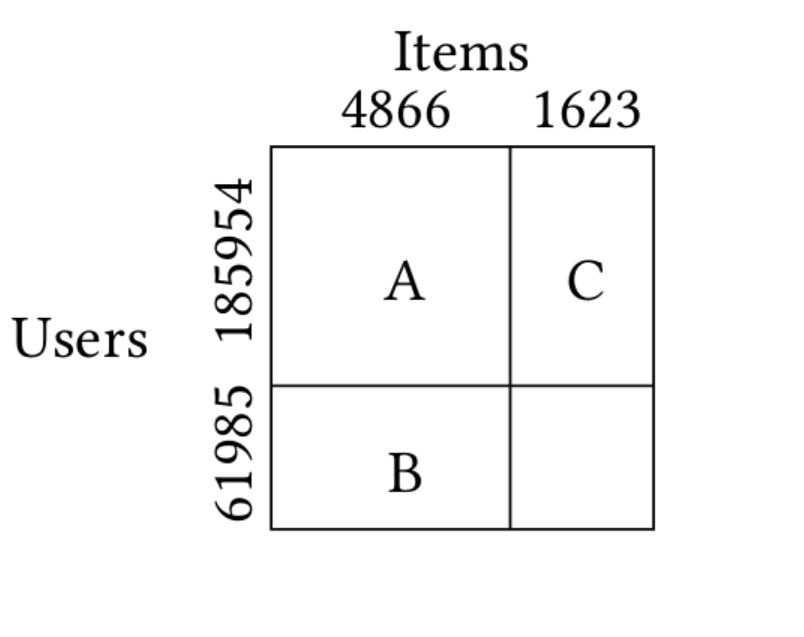
\includegraphics[width=0.3\textwidth]{figure}
\end{figure}
\textit{Discussion.} Let us discuss the new-item scenario first, since it
is the main focus of our work. In Table \ref{tab1}, we report the accuracy
metrics for different recommendation list sizes \textit{N}. LFW consistently
outperforms all the baselines in all metrics at any value of \textit{N} . We
want to highlight that LFW differs from the other CBF baselines
solely in the feature weighing scheme. Therefore, the improvement
in performance must be due to a better feature weighing discovered
by our approach.

In Table \ref{tab2}, we report the results for the item warm-start scenario.
For space reasons, we report only the values for \textit{N} = 5. As expected,
the CF approach based on SLIM has the best predictive accuracy
in the warm-start scenario. Interestingly, LFW still outperforms
both Cosine and Cosine TF-IDF baselines by a even large margin
with respect to the new item scenario. In summary, LFW cannot
compete with SLIM in warm-start scenarios, also due to its CBF
nature. Still, its degradation in performance is much less evident
than the other CBF baselines.

\begin{table}[ht]
    \centering
    \caption{Performance evaluation for the new-item scenario.}
    \label{tab1}
    \setlength{\tabcolsep}{2pt}
    \begin{tabular}{ccccccc}
        \hline
        Algorithm & n  & Precision       & Recall          & MRR             & MAP             & NCDG            \\ \hline
            & 5  & \textbf{0.1323} & \textbf{0.0825} & \textbf{0.2551} & \textbf{0.1062} & \textbf{0.0940} \\
        LFW       & 25 & \textbf{0.0858} & \textbf{0.2406} & \textbf{0.2795} & \textbf{0.0915} &     \textbf{0.1715} \\
          & 50 & \textbf{0.0654} & \textbf{0.3459} & \textbf{0.2822} & \textbf{0.0950} & \textbf{0.2097} \\
          &    &                 &                 &                 &                 &                 \\
          & 5  & 0.0938          & 0.0502          & 0.1984          & 0.0748          & 0.0622          \\
        Cosine    & 25 & 0.0624          & 0.1473          & 0.2189          & 0.0573          & 0.1127          \\
          & 50 & 0.0485          & 0.2231          & 0.2218          & 0.0582          & 0.1411          \\
          &    &                 &                 &                 &                 &                 \\
          & 5  & 0.0950          & 0.0533          & 0.2068          & 0.0752          & 0.0654          \\
        CosineIDF & 25 & 0.0658          & 0.1564          & 0.2280          & 0.0605          & 0.1192          \\
          & 50 & 0.0510          & 0.2348          & 0.2309          & 0.0621          & 0.1486          \\ \hline
\end{tabular}
\end{table}

\begin{table}[ht]
    \centering
    \caption{Performance evaluation for the warm-start scenario.}
    \label{tab2}
    \setlength{\tabcolsep}{2pt}
    \begin{tabular}{ccccccc}
\hline
Algorithm & n & Precision       & Recall          & MRR             & MAP             & NCDG            \\ \hline
SLIM      & 5 & \textbf{0.1383} & \textbf{0.1497} & \textbf{0.2819} & \textbf{0.1342} & \textbf{0.1453} \\
LFW       & 5 & \underline{ 0.0640}    & \underline{0.0577}    & \underline{0.1438}    & \underline{0.0744}          & \underline{0.0597}          \\ 
Cosine    & 5 & 0.0334          & 0.0277          & 0.0826          & 0.0270          & 0.0302          \\
CosineIDF & 5 & 0.0337          & 0.0258          & 0.0855          & 0.0276          & 0.0296          \\ \hline
\end{tabular}
\end{table}

\begin{table}[ht]
    \centering
    \caption{Evaluation of coverage and diversity.}
    \label{tab3}
    \setlength{\tabcolsep}{3pt}
    \begin{tabular}{ccccc}
        \hline
        Algorithm &                 \multicolumn{2}{c}{new-item}                 &                 \multicolumn{2}{c}{warm-start}\\
          & Coverage        & \multicolumn{1}{l|}{Diversity}             & Coverage        & Diversity       \\ \hline
        SLIM      & -               & \multicolumn{1}{l|}{-}                     & 0.1683          & \textbf{4.0585} \\
        LFW       & \underline{0.8897}    & \multicolumn{1}{l|}{\underline{\textbf{5.3628}}} & \underline{0.4891}    & \underline{2.1289}    \\
        Cosine    & 0.9236          & \multicolumn{1}{l|}{4.1529}                & \textbf{0.5723} & 1.1519          \\
        CosineIDF & \textbf{0.9495} & \multicolumn{1}{l|}{4.2061}                & 0.5684          & 1.1517          \\ \hline
\end{tabular}
\end{table}

In Table \ref{tab3}, we report the evaluation of coverage and diversity for
the top-5 recommendations in both scenarios. In the warm-start scenario,
``traditional'' CBF algorithms have greater coverage than CF,
whereas CF has greater diversity in the warm-start scenario. nterestingly,
LFW seems to ``take the best'' from both worlds, achieving
CBF-level coverage and CF-level diversity in both scenarios.

\section{QUALITATIVE ANALYSIS}
The good performances in both scenarios suggest that the weight
vector \textbf{w}* is capable of highlighting the importance of the various
features in terms of the user-perceived similarity. In order to understand
this concept better, we provide a qualitative analysis on how
features are weighted differently by two methods, namely Cosine
TF-IDF and our method LFW.

In Table \ref{tab4}, we report the highest and lowest weighted features
by LFW. For example, Jay Roach is the director of both “Meet the
Parents” and ``Meet the Fockers'', and of the Austin Powers series.
All these movies are comedy and target roughly the same audience,
hence they are good candidates of being recommended by a CF
algorithm despite having very different casts. Lois Maxwell has
acted as Miss Moneypenny – James Bond’s secretary – in the first
14 Bond movies. Hence, she represents another important cluster
of movies. Interestingly, Lois Maxwell has higher importance than
the various directors or main characters of Bond movies, since
they changed frequently among them. On the other hand, the
feature “snakebite” hardly identifies similar movies
 (for example, it
is shared by completely different movies like ``Kill Bill: Vol. 2'' and
``Siddharta''). Analogously, the feature “giant spider” is shared by
two masterpieces (``The Lord of the Rings'' and ``Harry Potter'') and
a collection of 12 minor unrelated movies.

\begin{table}[ht]
    \centering
    \caption{Features relevance learned by LFW. }
    \label{tab4}
    \begin{tabular}{cc}
        \hline
        Most relevant features & Least relevant features \\ \hline
        Molly Ringwald         & snakebite               \\
        Jay Roach              & John Ashton             \\
        Lois Maxwell           & Ally Sheedy             \\
        motorcycle accident    & giant spider            \\
        Jayne Eastwood         & stable                  \\ \hline
    \end{tabular}
\end{table}

Table \ref{tab5} shows that TF-IDF, by weighing features proportionally
to their rarity, can hardly capture any interesting relationship from
the actual movie consumption. Surprisingly, features representing
genres (such as comedy and thriller) have low weights.

To shed a light on this, in Table \ref{tab6} we report the features that
differ the most between LFW and TF-IDF. The weights vectors of
both methods were first normalized in [0, 1] before computing their
difference feature-wise. It is interesting to see that LFW raises the
relevance of genres w.r.t. TF-IDF, which are definitely an important
set of features that receive a really low TF-IDF weight. Conversely,
the relevance of very rare countries of origin in our dataset (e.g.
Brazil and Romania) is strongly decreased. For example, we have
only 2 Brazilian movies with just 20 ratings in common in our
dataset.

\begin{table}[ht]
    \centering
    \caption{Features relevance according to TF-IDF.}
    \label{tab5}
    \begin{tabular}{cc}
        \hline
        Most relevant features & Least relevant features \\ \hline
        knowledge              & drama                   \\
        Iran                   & comedy                  \\
        Bulgaria               & film independent        \\
        China                  & thriller                \\
        Argentina              & romance                 \\ \hline
    \end{tabular}
\end{table}

\begin{table}[ht]
    \centering
    \caption{Feature importance LFW vs TF-IDF.}
    \label{tab6}
    \begin{tabular}{cc}
        \hline
        LFW \textgreater{}TF-IDF & LFW \textless TF-IDF \\ \hline
        USA                      & Brazil               \\
        drama                    & Romania              \\
        Molly Ringwald           & Peru                 \\
        comedy                   & Philippines          \\
        film independent         & George P. Cosmatos   \\ \hline
    \end{tabular}
\end{table}

\section{CONCLUSION AND FUTURE WORK}
In this paper, we propose a feature-based linear regression framework 
for personalized recommendation. We presented a novel approach 
to compute item feature scores that defines their relevance
according to expressed user preferences. In contrast to traditional
recommender systems, our approach solves both the item and the
user cold start issues. Moreover, it has a linear temporal complexity
with respect to item features, and thus it is lighter than the
state of the art competitor models. Future directions include the
development of personalized feature weighing tools and the extensive 
evaluation of this approaches with different datasets and CF
algorithms.

\bibliographystyle{abbrv}
\bibliography{zdroje}

\balancecolumns

\end{document}
